\documentclass[12pt]{report}
\usepackage[utf8]{inputenc}
\usepackage{amsmath}
\usepackage{graphicx}
\graphicspath{ {./include/} }
\usepackage{float}
\usepackage{hyperref}
\usepackage{xcolor}
\usepackage{listings}
\usepackage{caption}
\DeclareCaptionFont{white}{\color{white}}
\DeclareCaptionFormat{listing}{%
	\parbox{\textwidth}{\colorbox{gray}{\parbox{\textwidth}{#1#2#3}}\vskip-4pt}}
\captionsetup[lstlisting]{format=listing,labelfont=white,textfont=white}
\lstset{frame=lrb,xleftmargin=\fboxsep,xrightmargin=-\fboxsep}

%opening
\title{Radiative Correction Framework\\ A Quick Start Guide}
\author{Fady Shaker}


\begin{document}

\maketitle
\tableofcontents
\newpage
\section{Introduction}
This document will walk you through how to use and modify the radiative correction framework starting from creating the particle guns till producing the efficiency ratios required for a fake data study.\\

The full code is accessible at:\\
\url{https://github.com/f-shaker/radiative_correction}\\
and the generated root files for the analysis are available at:\\
\url{https://yuoffice-my.sharepoint.com/:f:/r/personal/fshaker_yorku_ca/Documents/radcorr_root_files?csf=1&web=1&e=BsrP6P}

\subsection{Framework Overview}
\begin{figure}[!ht]
	\center{
	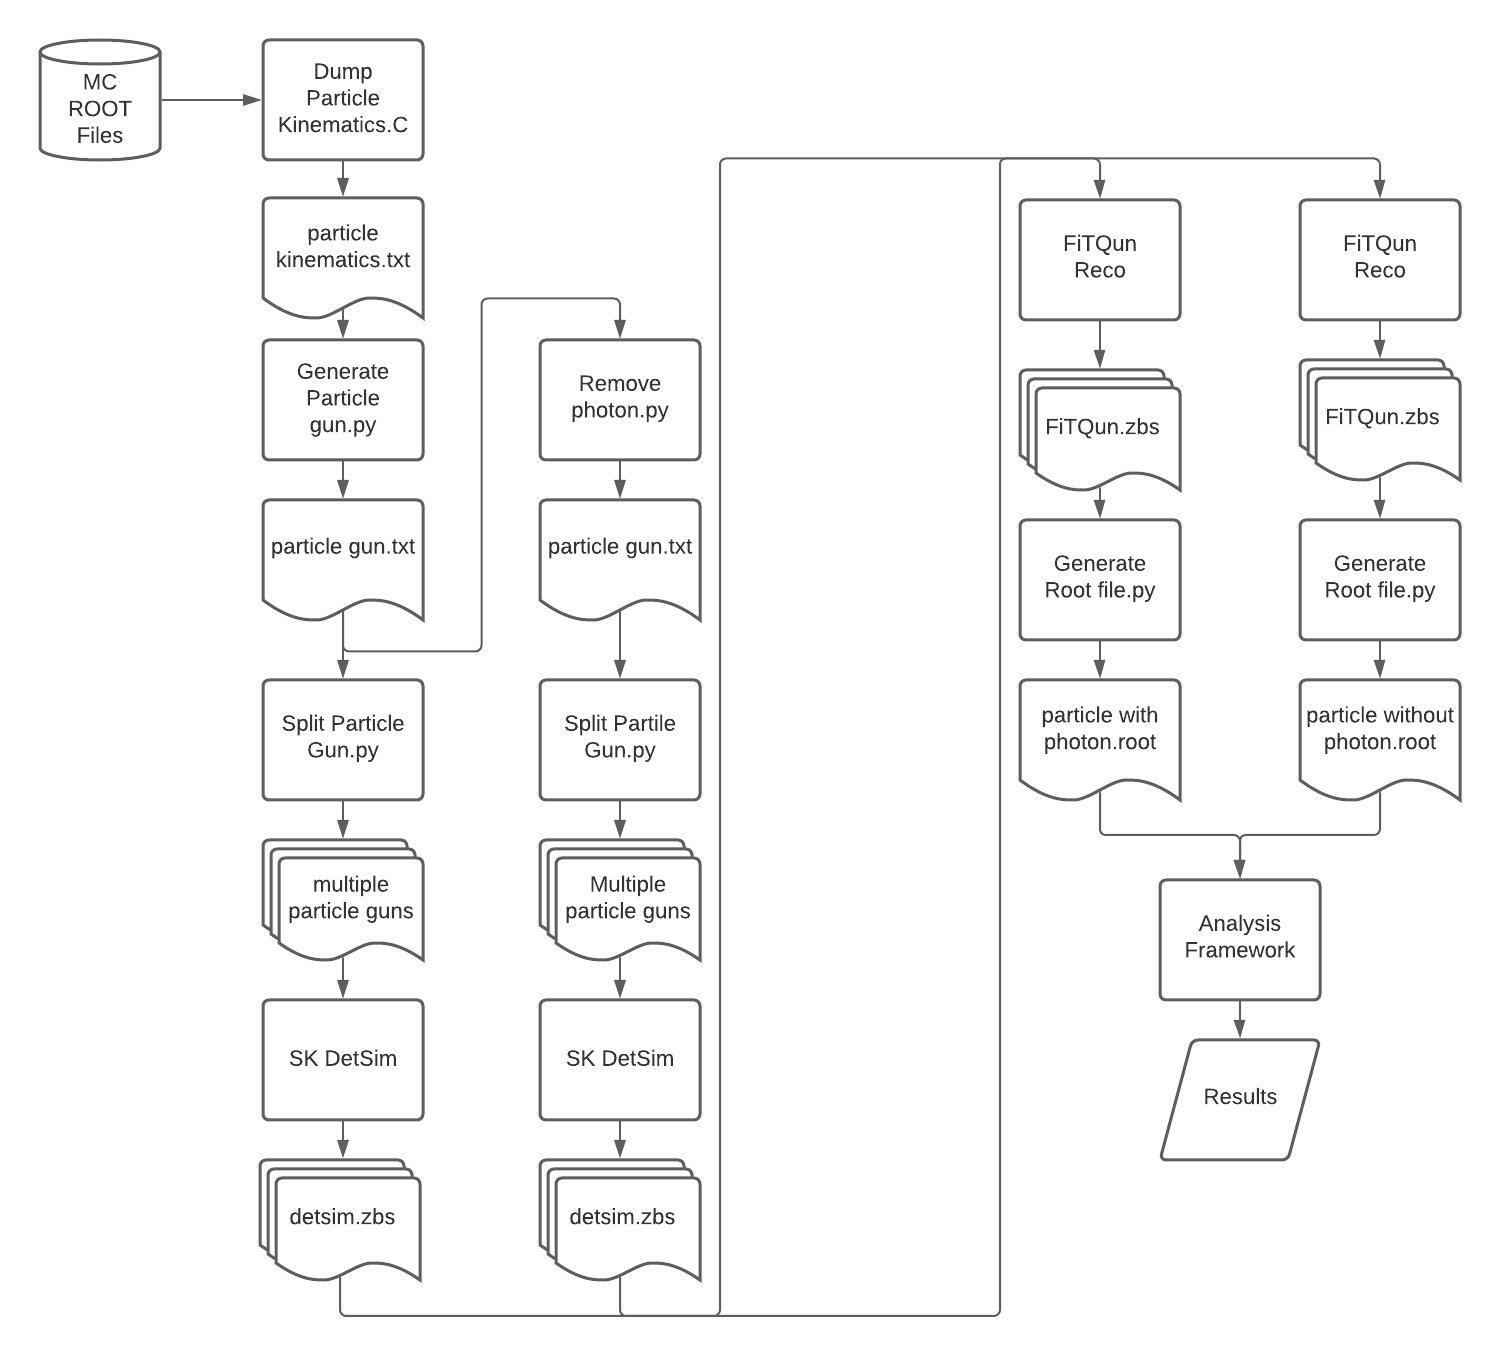
\includegraphics[scale=0.5]{radcorr_sw_framework.jpeg}
	\caption{Radiative Correction Framework}	
	}
\end{figure}
\section{Creating a Particle Gun}
\subsection{Dumping Particle Kinematics}
In order to create a realistic particle gun, covering the full SK detector volume, the vertex position and output lepton ($\mu^-$, $e^-$, $\mu^+$, $e^+$) kinematics are read for the unoscillated SK MC files. This operation is done on two steps:\\
\begin{enumerate}
	\item Adding the MC files to create a single root file through hadd\\
\begin{lstlisting}[language=Python, caption=Combining MC ROOT files]
python hadd_nu.py --particle=<particle type>							
\end{lstlisting}
where $<$particle type$>$ can  be ``nue", ``nuebar", ``numu" or ``numubar" .
	\item Dump the content of the single root file into a text file containing the vertex position of a specific interaction (NEUT code) and output lepton total energy and direction. 
Change the dump\_particle\_kinematics.C configurations (e.g. input and output files). Then, from ROOT run
\begin{lstlisting}[language=C++, caption=Dumping Particle Kinematics]
dump_particle_kinematics(particle_pdg)	
\end{lstlisting}	
\end{enumerate}
At the end of this step, we will have a text file with the following format:\\
Energy dir\_x dir\_y dir\_z vertex\_x vertex\_y vertex\_z 	
\subsection{Adding the Photon}
The particle kinematics produced from the above step, does not contain any photons. Now, we will add a photon associated with that lepton at the same vertex and conserve energy, so the final output lepton energy = initial output lepton energy + photon energy. 
\section{ROOT Analysis}
\subsection{Creating the Weight Branches}
The main idea is to merge the two root files: lepton kinematics with photons (radiative) and lepton kinematics without photon (non-radiative) to produce a realistic particle gun. The created mixed-weighted root file must, at least, has a new branch that indicate if this event is radiative or not. It can also calculate the correct radiative (non-radiative) weight as well as the oscillation probabilities. However this functionality is currently overwritten in the main code.
To produce the mixed weight files, use the following function 
\begin{lstlisting}[language=C++, caption=Creating Weight Branch Example]
/*void create_weight_branches(std::string in_file_name,
bool is_sim_gamma,
fq_particle i_particle,
bool is_antiparticle)
*/
create_weight_branches("muplus_ginft180_5e4.root",
true, MUON, true);
create_weight_branches("muplus_init_5e4.root",
false, MUON, true);
/* then use hadd -f muplus_g_weighted.root
muplus_ginft180_5e4.root muplus_init_5e4.root */							
\end{lstlisting} 



\begin{thebibliography}{9}
	\bibitem{Ko_phd} 
	Konosuke Iwamoto. 
	\textit{Neutrino Oscillation Measurements with An Expanded Electron Neutrino Appearance Sample in T2K, 2017.}
	
	%	\bibitem{Pueh_msc} 
	%	Pueh Leng Tan.
	%	\textit{Study of QED radiative corrections to
	%		charged lepton leg in neutrino-nucleon
	%		interactions, 2013.} 
	
	\bibitem{Kevin_talk1} 
	Kevin McFarland and Konosuke Iwamoto.
	\textit{Radiative CCQE and T2k's Oscillation Analyses, 2018}
	
	\bibitem{Rujula_calc}
	A. De Rujula, R. Petronzio and A. Savoy-Navarro
	\textit{Radiative Corrections to High-Energy Neutrino Scattering. Nucl.Phys. B154 (1979) 394. CERN-TH-2593.}
	
\end{thebibliography}
	
\end{document}

